\documentclass[UTF8,aspectratio=169]{ctexbeamer}
\usetheme{Madrid}
\usecolortheme{default}
\usepackage{amsmath}
\usepackage{booktabs}
\usepackage{array}
\usepackage{xcolor}
\usepackage{xurl}
\usepackage{colortbl}
\usepackage{graphicx}

\newcommand{\good}[1]{\textcolor{green!45!black}{#1}}
\newcommand{\warn}[1]{\textcolor{red!65!black}{#1}}
\newcommand{\bluenote}[1]{\textcolor{blue!65!black}{#1}}
\newcolumntype{L}[1]{>{\raggedright\arraybackslash}p{#1}}
\definecolor{winrow}{RGB}{220,240,220}
\definecolor{softrow}{RGB}{232,242,255}
\definecolor{warnrow}{RGB}{250,228,228}

% Recurring roadmap so the narrative thread stays visible.
\AtBeginSection[]{%
  \begin{frame}{Roadmap}
    \footnotesize
    \tableofcontents[currentsection, hideallsubsections]
  \end{frame}}

\title[Residual Family Head]{Residual Family Head: Making the Deployed Surrogate Extensible}
\subtitle{Additive residual on a frozen backbone --- and how far a cheap per-family adapter goes}
\author{Mie Spray Postprocessing Project}
\date{2026-06-01}

\begin{document}

\begin{frame}
  \titlepage
\end{frame}

% ------------------------------------------------------------------
\begin{frame}{The thread of this deck}
\small
We take the deployed Stage-3 surrogate from Chapter~5 and ask one question:
\begin{center}
\emph{can we make it extensible to new injector families \textbf{without} giving up
accuracy --- and how far does the cheap adapter reach?}
\end{center}

\vspace{0.4em}
\textbf{One principle ties every experiment together:}
\[
  \boxed{\ \text{prediction} \;=\; \underbrace{\text{shared backbone}}_{\text{frozen, hot-started}}
  \;+\; \underbrace{\text{small per-family residual}}_{\text{trained, zero-initialised}}\ }
\]

\vspace{0.4em}
\begin{enumerate}\setlength\itemsep{2pt}
  \item \textbf{Where Chapter 5 leaves off} --- two open gaps.
  \item \textbf{Theory} --- additive residual on a frozen backbone.
  \item \textbf{In-distribution climb} --- residual head $\to$ FiLM $\to$ multi-task SVGP.
  \item \textbf{Robustness} --- LONO transfer and dataset-sensitivity checks.
  \item \textbf{Boundary} --- where the cheap adapter stops working.
  \item \textbf{Significance} --- what this changes about the thesis conclusions.
\end{enumerate}
\end{frame}

% ==================================================================
\section{Where Chapter 5 leaves off}

% ------------------------------------------------------------------
\begin{frame}{Where the thesis leaves the surrogate}
\small
Chapter~5 reports a three-stage MLP screening surrogate and an SVGP alternative
backbone on the \textbf{conservative uncensored CDF table} (542{,}565 points).
This is the \emph{same table} the residual study uses --- anchored by the SVGP,
which scores \textbf{4.193 mm} in both documents.

\vspace{0.3em}
\begin{center}
\renewcommand{\arraystretch}{1.15}
\setlength{\tabcolsep}{6pt}
\begin{tabular}{@{}lrr@{}}
\toprule
\textbf{Model (uncensored CDF, 542k pts)} & \textbf{RMSE [mm]} & \textbf{P50 RMSE [mm]} \\
\midrule
Calibrated Hiroyasu--Arai (physics)      & 10.261 & -- \\
Naber--Siebers w/ delay (physics)        & \phantom{0}9.286 & -- \\
Three-stage MLP, selected surrogate (5-seed) & \phantom{0}4.265 & 2.848 \\
\rowcolor{softrow}
Stage-3 SVGP (thesis' strongest predictor) & \textbf{\phantom{0}4.193} & \textbf{2.649} \\
\bottomrule
\end{tabular}
\end{center}

\vspace{0.4em}
\footnotesize
The thesis verdict is deliberately \emph{not} a single winner: the SVGP wins point
accuracy and LONO transfer; the MLP is kept as a conservative in-domain surrogate
with an auditable workflow and an injection-onset head. LONO is fragile on
\textbf{Nozzle0}, the only first-generation injector --- a cross-design-family
extrapolation failure.
\end{frame}

% ------------------------------------------------------------------
\begin{frame}{Two open problems the thesis does not close}
\small
\begin{columns}[T]
\column{0.5\textwidth}
\begin{block}{1. Deployment / extensibility}
The deployed model conditions on injector family. To add a \emph{new} family it
needs either a hard-coded fallback identity or a freshly trained head. There is no
clean, structural answer for an unseen injector.
\end{block}

\column{0.5\textwidth}
\begin{block}{2. Accuracy frontier}
The best single model on the primary table is the SVGP at 4.193 mm. Can the same
censoring-aware protocol be pushed further \emph{without} abandoning the deployed
backbone?
\end{block}
\end{columns}

\vspace{0.6em}
\textbf{Claim of this study.} Converting the deployed family-aware Stage-3 model into a
\emph{residual family head}
\[
  \mu(x,f) = \mu_{\rm shared}(h(x)) + \Delta_f(h(x))
\]
addresses \emph{both}: it gives a structural new-family fallback \textbf{and}, on the
SVGP backbone, sets a new best on the primary table --- while every variant
hot-starts from the deployed checkpoint and freezes its trunk.
\end{frame}

% ==================================================================
\section{Theory: additive residual on a frozen backbone}

% ------------------------------------------------------------------
\begin{frame}{Conditioning on injector family: three designs}
\small
Let $h(x)$ be the shared trunk representation of the low-dimensional condition
descriptor $x$ (time, $A$-scaled amplitude, log-pressure residual). Family $f$ can
enter the mean in three ways:

\vspace{0.2em}
\begin{center}
\renewcommand{\arraystretch}{1.25}
\setlength{\tabcolsep}{4pt}
\begin{tabular}{@{}L{3.3cm}L{4.4cm}L{2.8cm}r@{}}
\toprule
\textbf{Design} & \textbf{Family signal} & \textbf{New family} & \textbf{CDF RMSE} \\
\midrule
One-hot input & feature into one shared head $\mu(h,f)$ & implicit & 4.265 \\
\rowcolor{warnrow}
Per-family head & each family owns a decoder $\mu_f(h)$ & \warn{needs fallback / trained head} & 5.056 \\
\rowcolor{winrow}
Residual head & shared mean $+$ small residual $\mu_{\rm shared}+\Delta_f$ & \good{zero residual $\to$ shared} & 4.631 \\
\bottomrule
\end{tabular}
\end{center}

\vspace{0.15em}
\begin{itemize}\setlength\itemsep{1pt}
  \item The deployed \textbf{per-family head} buys per-family capacity but
        \warn{fragments the data} --- aggregate RMSE rises to 5.056 vs the
        single-head surrogate's 4.265 --- \emph{and} leaves no answer for an unseen family.
  \item The \textbf{residual head} recovers most of that lost accuracy
        \good{(5.056$\to$4.631)} while making the fallback \emph{structural}.
\end{itemize}
\end{frame}

% ------------------------------------------------------------------
\begin{frame}{Residual head: identity warm-start + structural fallback}
\small
\begin{columns}[T]
\column{0.55\textwidth}
\[
  \mu(x,f) = \mu_{\rm shared}(h(x)) + \Delta_f(h(x)),\qquad \Delta_f\!\equiv\!0\ \text{at init}
\]
\textbf{Residual-learning view.} Like a residual block, each family learns a
\emph{correction} to a strong shared predictor, not the whole map. Zero-initialised
$\Delta_f$ means the model \emph{equals} the deployed production model at step~0;
training only perturbs it.

\vspace{0.25em}
\textbf{Structural fallback.} An unseen family carries $\Delta_f\equiv 0$, so it
\emph{naturally} predicts $\mu_{\rm shared}$ --- no hard-coded
\texttt{fallback\_family\_id}.

\vspace{0.25em}
\textbf{Shrinkage prior.} The $\Delta_f$ weight-decay (\texttt{delta\_L2}) is an
explicit prior pulling each family back toward the shared model --- hierarchical
shrinkage trading per-family fit against shared-model proximity.

\column{0.45\textwidth}
\footnotesize
\begin{block}{Parameter-efficient transfer}
Freeze the backbone, train only tiny per-family modules:
\begin{itemize}\setlength\itemsep{1pt}
  \item trunk frozen: 334{,}720 params
  \item shared mean frozen: 16{,}641 params
  \item \good{trainable: 49{,}923} ($\Delta$ heads $+$ log-var)
\end{itemize}
The adapter / PEFT paradigm: a frozen backbone plus tiny task heads, so a new
family is a new adapter --- not a retrain.
\end{block}

\begin{block}{Warm-start mapping}
\scriptsize
copy \texttt{trunk.*}; copy \texttt{log\_var\_head.*};
\texttt{mu\_heads.1}$\to$\texttt{mu\_shared\_head};
\texttt{delta\_heads.*} zero-init, then 10-epoch KD mimic.
\end{block}
\end{columns}
\end{frame}

% ------------------------------------------------------------------
\begin{frame}{Two richer instantiations of the same principle}
\small
\begin{block}{FiLM: condition the \emph{representation}, not just the offset}
\[
  h_l' = \gamma_{f,l}\odot h_l + \beta_{f,l},\qquad
  \mu(x,f)=\mu_{\rm shared}(h_L')+\Delta_f(h_L')
\]
Feature-wise linear modulation inserts a per-family affine transform \emph{inside}
the trunk. Identity init ($\gamma=1,\beta=0,\Delta_f=0$) preserves the exact
warm-start. It asks: does injector family change \emph{how} $(a,\Delta p)$ are
represented, or only the final mean offset?
\end{block}

\begin{block}{Additive-residual multi-task SVGP: the same idea on a GP backbone}
\[
  g(x,f) = g_{\rm shared}(x) + \delta_f(x)
\]
A shared sparse variational GP hot-started from the deployed Stage-3 SVGP, plus a
per-family residual GP. Family id \emph{routes} the residual but stays out of the
kernel feature vector; an unseen family falls back to $g_{\rm shared}$. This is a
shared-plus-per-family \emph{additive (hierarchical)} multi-task GP; its
probabilistic backbone yields the best-calibrated residual variant in this study
(ECE \good{0.026}).
\end{block}

\vspace{0.2em}
\footnotesize
All three share the contract: \textbf{hot-start the deployed checkpoint, freeze the
backbone, train only zero-/identity-initialised per-family residuals.}
\end{frame}

% ------------------------------------------------------------------
\begin{frame}{Architecture: Family Head vs Residual vs FiLM}
\small
\begin{center}

\includegraphics[width=0.96\textwidth]{figs/mlp_family_conditioning_architecture.png}
\end{center}
\vspace{-0.2em}
\footnotesize
\centering
Left: per-family decoders. Middle: shared mean $+$ zero-init residual.
Right: last-block identity FiLM $+$ residual head; production refinement freezes the
trunk and shared-mean head, then updates FiLM, residual, and log-variance heads.
\end{frame}

% ------------------------------------------------------------------
\begin{frame}{Experiment contract}
\small
\begin{block}{Fixed production baseline}
\begin{itemize}\setlength\itemsep{2pt}
  \item Baseline run:
        \texttt{distill\_cdf\_family\_head\_v3\_FROZEN\_anchor\_off\_20260529\_213346}
        (the deployed per-family-head model, CDF RMSE 5.056).
  \item Feature contract: \texttt{a\_dp050\_plus\_pressures}; device CUDA;
        seed inherited from the production run.
  \item Evaluation: canonical point tables
        (\texttt{cdf\_uncensored}, \texttt{p50\_observed}, \texttt{q1\_grid\_all}) ---
        \texttt{cdf\_uncensored} is the thesis' 542k-point primary table.
\end{itemize}
\end{block}

\vspace{0.3em}
\begin{center}
\renewcommand{\arraystretch}{1.15}
\begin{tabular}{@{}L{4.0cm}L{8.6cm}@{}}
\toprule
\textbf{Knob} & \textbf{Values} \\
\midrule
Residual shrinkage & \texttt{0}, \texttt{1e-4}, \texttt{1e-3}, \texttt{1e-2} \\
Mimic warm-up & 10 epochs; teacher is the deployed production model \\
Refinement & 150 max epochs, patience 20, trunk frozen \\
Trainable params & 49{,}923: residual deltas $+$ shared log-var head \\
\bottomrule
\end{tabular}
\end{center}
\end{frame}

% ==================================================================
\section{In-distribution climb}

% ------------------------------------------------------------------
% Compressed training/result summary: one page, three figures + one-line verdict.
\begin{frame}{Systematic family differences $\Rightarrow$ residual fine-tune works}
\small
\begin{columns}[T,onlytextwidth]
\column{0.34\textwidth}
\centering

\includegraphics[width=\linewidth,height=0.52\textheight,keepaspectratio]{figs/injector_scatter_all_nozzles.png}\\[0.3em]
{\scriptsize \textbf{The data} --- all nozzles, dimensionless penetration: the injector families separate \emph{systematically}, not by noise.}
\column{0.34\textwidth}
\centering

\includegraphics[width=\linewidth,height=0.52\textheight,keepaspectratio]{figs/mlp_family_conditioning_architecture.png}\\[0.3em]
{\scriptsize \textbf{The architecture} --- frozen backbone $+$ zero-init per-family residual (Family Head / Residual / FiLM); unseen family $\to$ shared model.}
\column{0.32\textwidth}
\centering
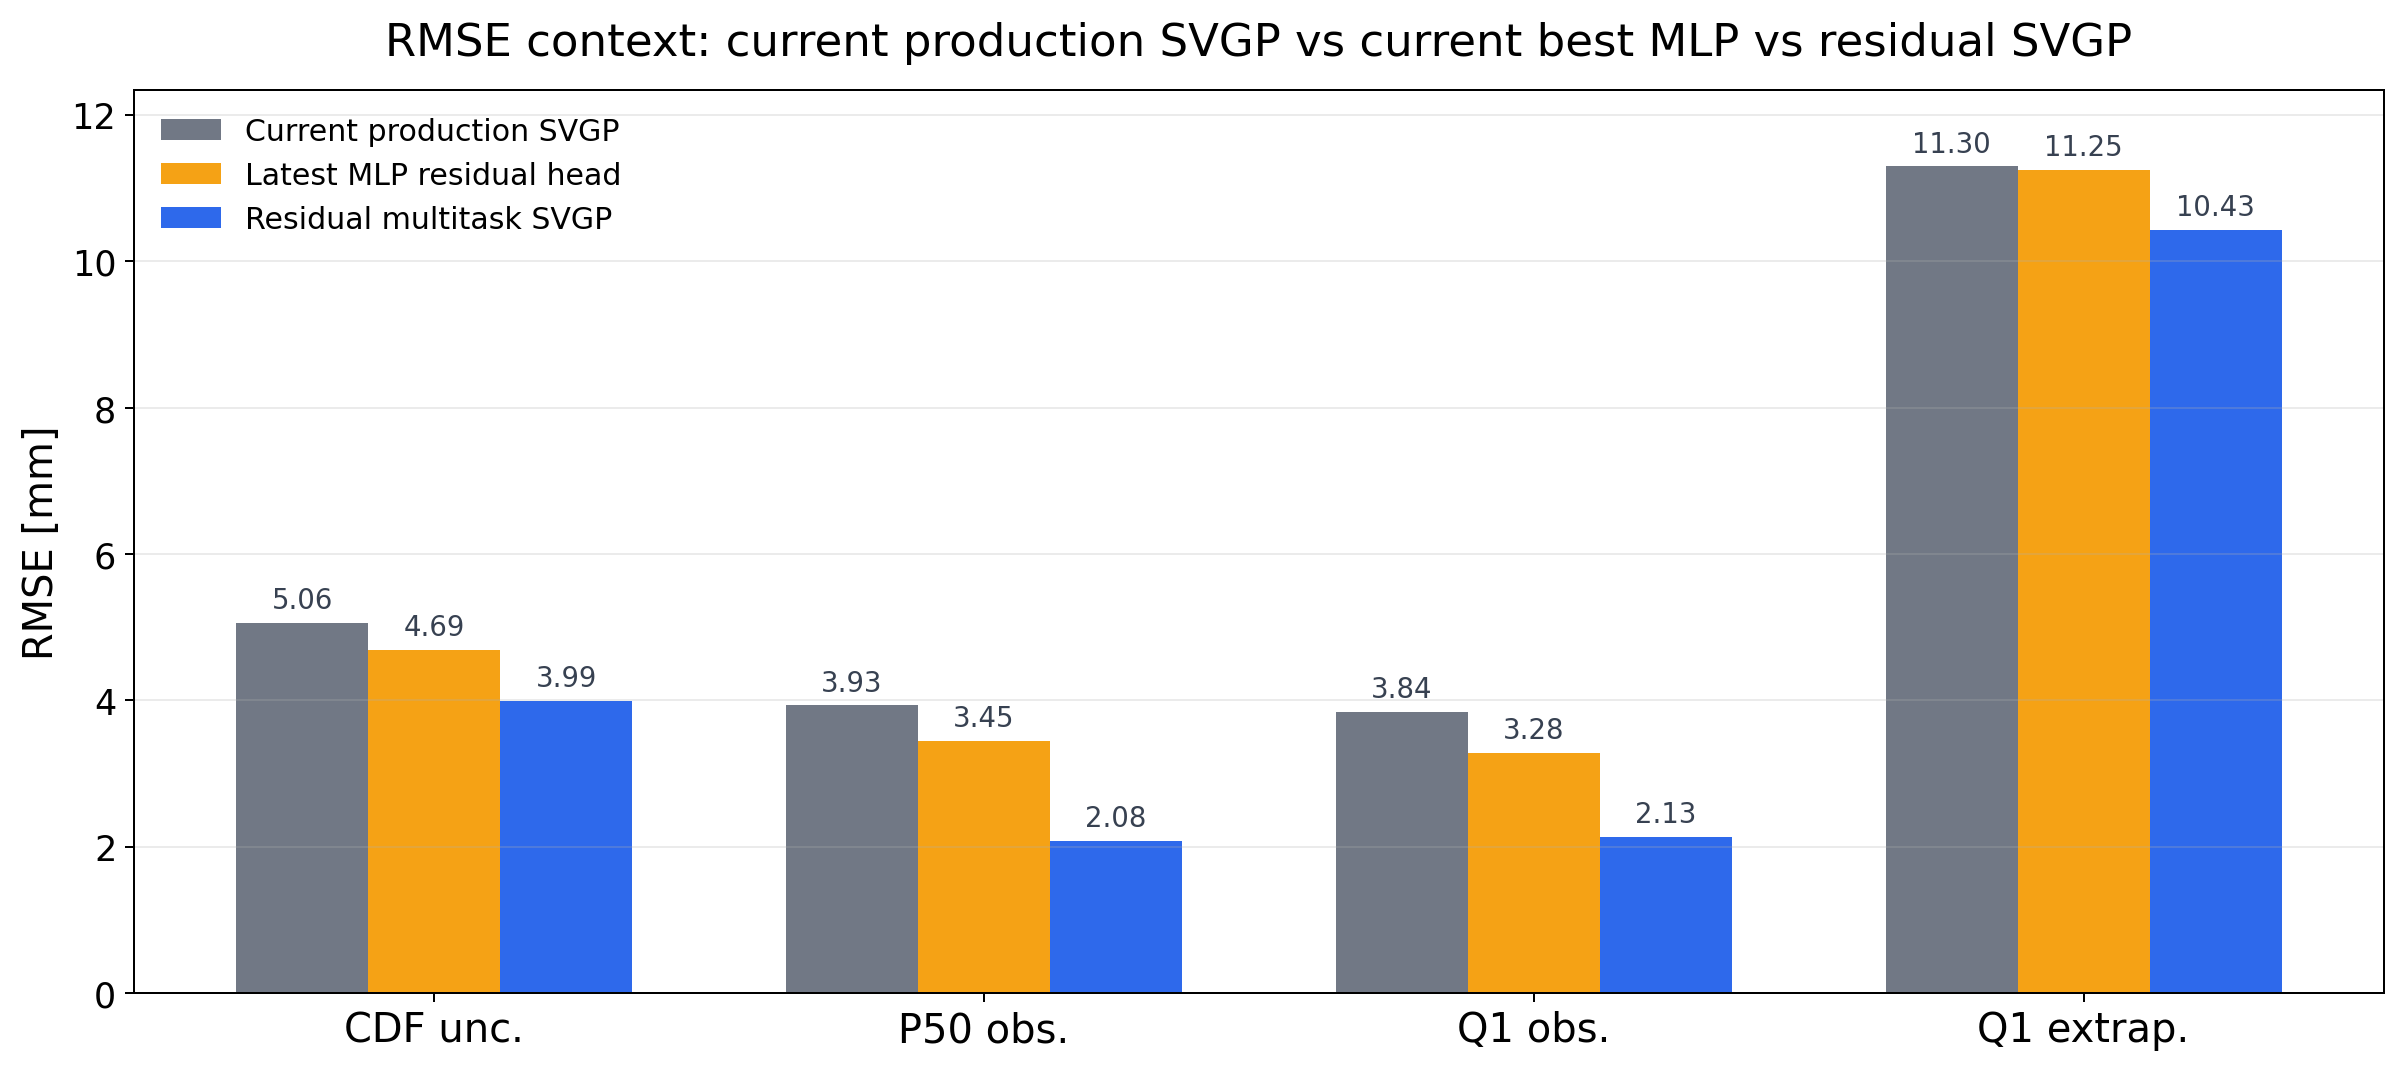
\includegraphics[width=\linewidth,height=0.52\textheight,keepaspectratio]{figs/residual_svgp_context_rmse_comparison.png}\\[0.3em]
{\scriptsize \textbf{The result} --- the residual fine-tune lowers RMSE across CDF / P50 / Q1 vs the deployed model.}
\end{columns}
\vspace{0.4em}
\begin{center}\large\good{The data proves the systematic difference is real, and the residual fine-tune works.}\end{center}
\end{frame}

% ==================================================================
\section{Robustness: LONO and dataset sensitivity}

% ------------------------------------------------------------------
\begin{frame}{LONO: does the residual win survive an unseen nozzle?}
\small
\begin{block}{Protocol}
\begin{itemize}\setlength\itemsep{2pt}
  \item Hold out Nozzle 1, 2, 4, 5, 6 one at a time; \textbf{Nozzle0 stays in train}
        as the sole first-generation anchor (holding it out is a separate OOD study).
  \item Each fold trains Stage-1$\to$2$\to$3 \emph{from scratch} with the nozzle
        removed --- no production-checkpoint leakage.
  \item Arms: family-head teacher, residual FH (\texttt{1e-4}),
        residual-FiLM (\texttt{film 1e-4, delta 1e-3}).
\end{itemize}
\end{block}
\vspace{0.1em}
\begin{center}
\scriptsize
\renewcommand{\arraystretch}{1.14}
\setlength{\tabcolsep}{4.2pt}
\begin{tabular}{@{}lrrrr@{}}
\toprule
\textbf{Aggregation} & \textbf{Family head} & \textbf{Residual FH} & \textbf{Residual-FiLM} & \textbf{HA / NS} \\
\midrule
All 5 folds & 8.32 $\pm$ 2.33 & 6.95 $\pm$ 4.05 & 6.96 $\pm$ 4.08 & 11.69 / 11.10 \\
\rowcolor{winrow}
4 folds excl.\ N6 & 7.44 $\pm$ 1.46 & \textbf{5.16 $\pm$ 0.65} & \textbf{5.15 $\pm$ 0.67} & 11.93 / 11.37 \\
\bottomrule
\end{tabular}
\end{center}
\vspace{0.25em}
\footnotesize
On in-family folds the residual conversion cuts family-head RMSE by \good{31\%}
(7.44$\to$5.16) and nearly halves the fold spread. N6 is reported as an OOD stress
fold, not hidden in the mean. (The thesis LONO holds out N0,1,2,4,5; here N0 stays
in as the family anchor and N6 is the in-protocol sparse/OOD fold --- N6 is not a
thesis fold.)
\end{frame}

% ------------------------------------------------------------------
\begin{frame}{LONO: per-fold read}
\small
\begin{center}
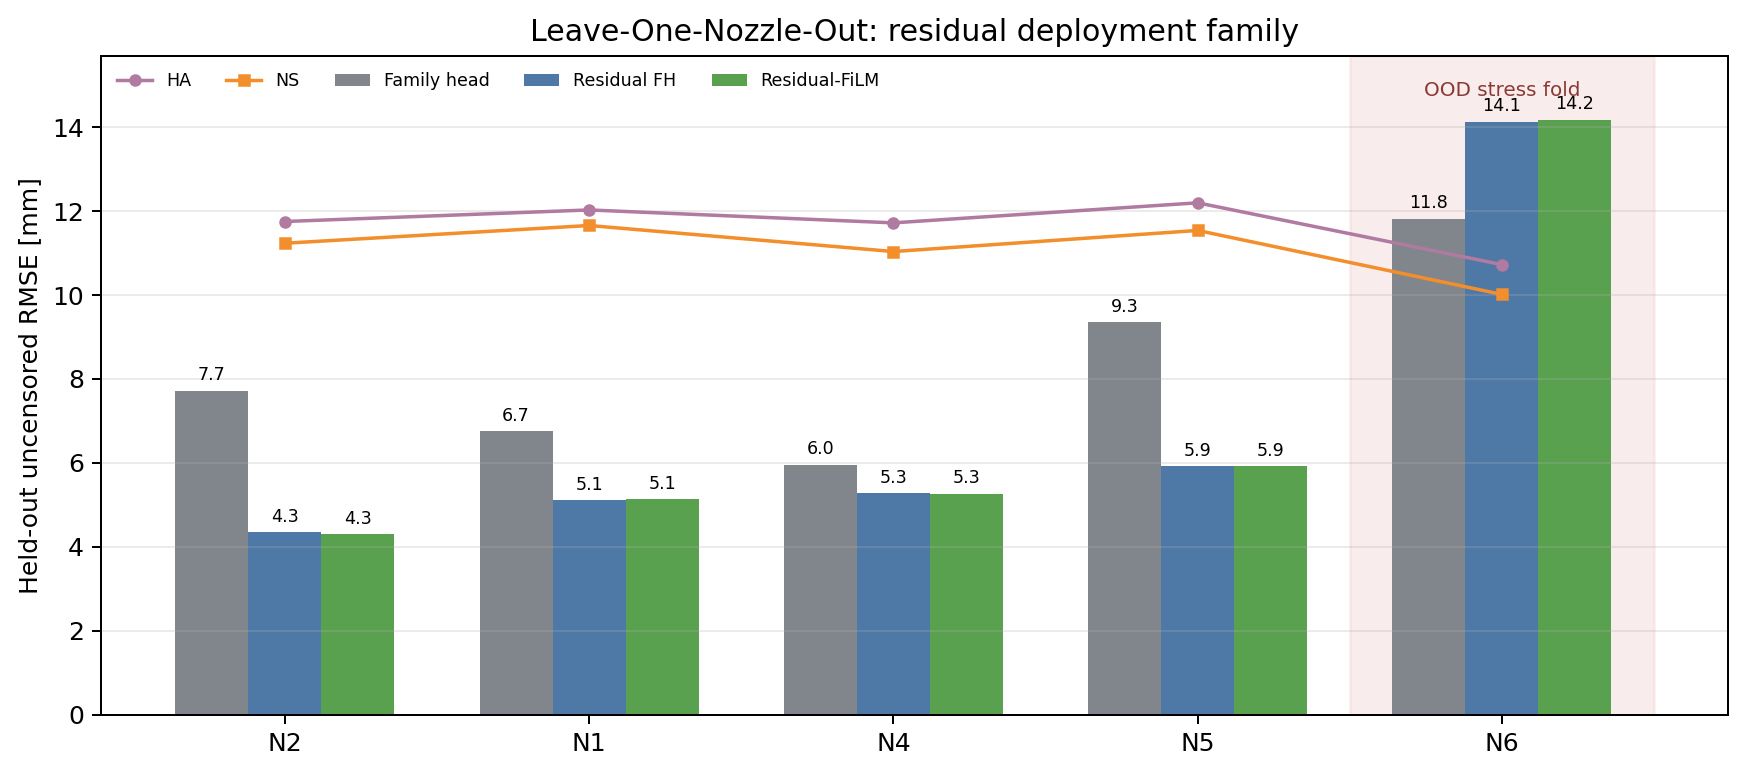
\includegraphics[width=0.92\textwidth]{figs/lono_modified_only_rmse_by_fold.png}
\end{center}
\vspace{-0.2em}
\footnotesize
\centering
Residual FH improves every in-family fold: N2 \good{$-3.37$}, N1 \good{$-1.64$},
N4 \good{$-0.68$}, N5 \good{$-3.43$} mm. N6 \warn{$+2.31$} (regression).
\end{frame}

% ------------------------------------------------------------------
\begin{frame}{LONO: verdict}
\small
\begin{itemize}\setlength\itemsep{3pt}
  \item \textbf{The residual deployment win generalises (MLP arms).} On all four
        in-family held-out nozzles the residual arms beat the family-head teacher and
        dominate the HA/NS physics baselines on nozzles they never trained on. (LONO
        here covers the MLP variants; the residual SVGP is not yet LONO-tested.)
  \item \textbf{Bias repair.} The family head over-predicts (+3 to +8 mm); the
        residual conversion moves the 4-fold mean bias from \(+5.07\) to
        \good{$+0.78$} mm and restores coverage (0.44$\to$0.78 on N5).
  \item \textbf{FH $\approx$ FiLM under LONO.} Per-fold numbers agree within 0.04 mm.
        FiLM's in-distribution edge does \emph{not} translate into unseen-nozzle
        transfer --- for a new nozzle, the cheap output residual is as good as the
        representation adapter.
  \item \textbf{N6 is a true stress fold.} All MLP arms collapse to 12--14 mm and the
        residual arms under-predict severely (bias $-10.5$). This foreshadows the
        Nozzle0 case and motivates a separate OOD study, not another adapter sweep.
\end{itemize}
\end{frame}

% ------------------------------------------------------------------
\begin{frame}{Dataset sensitivity matrix: explicit lv2 vs lv3 roots}
\small
\begin{center}
\scriptsize
\renewcommand{\arraystretch}{1.12}
\setlength{\tabcolsep}{4pt}
\begin{tabular}{@{}llrrrr@{}}
\toprule
\textbf{Model} & \textbf{Train root} & \textbf{lv2 CDF} & \textbf{lv3 CDF} & \textbf{lv2 P50} & \textbf{lv3 P50} \\
\midrule
Family head baseline & pre-QC & 5.010 & 4.901 & 3.907 & 3.785 \\
Residual FH          & pre-QC & 4.631 & 4.519 & 3.395 & 3.264 \\
Residual-FiLM        & pre-QC & 4.510 & 4.401 & 3.166 & 3.035 \\
Residual SVGP        & pre-QC & 3.987 & 3.921 & 2.077 & 2.026 \\
\rowcolor{winrow}
Residual SVGP        & lv3 QC & \textbf{3.922} & \textbf{3.848} & \textbf{1.912} & \textbf{1.829} \\
\bottomrule
\end{tabular}
\end{center}
\vspace{0.25em}
\footnotesize
\textbf{Controlled read:} every row is re-scored through an explicit
\texttt{--synthetic-root}; \texttt{MLP/synthetic\_data} is never used. The lv3 root is
a target/evaluation cleanup sensitivity check, so its lower RMSE is evidence of
robustness to cleaning choices, not a replacement for the lv2 primary comparison.
\end{frame}

% ------------------------------------------------------------------
\begin{frame}{QC-gated retrain: cleanup vs model gain}
\small
\begin{center}
\scriptsize
\renewcommand{\arraystretch}{1.12}
\setlength{\tabcolsep}{4pt}
\begin{tabular}{@{}lrrr@{}}
\toprule
\textbf{Model} & \textbf{Cleanup} & \textbf{QC retrain} & \textbf{Net} \\
 & \scriptsize old lv3 -- old lv2 & \scriptsize QC lv3 -- old lv3 & \scriptsize QC lv3 -- old lv2 \\
\midrule
Residual FH    & \good{-0.112} & \warn{+0.071} & -0.041 \\
Residual-FiLM  & \good{-0.108} & -0.001 & -0.109 \\
\rowcolor{winrow}
Residual SVGP  & \good{-0.067} & \good{-0.073} & \good{-0.140} \\
\bottomrule
\end{tabular}
\end{center}
\vspace{0.25em}
\footnotesize
\begin{itemize}\setlength\itemsep{2pt}
  \item \textbf{Post-training is the main structural move:} on lv2, family head
        $5.010\to$ residual FH 4.631 $\to$ FiLM 4.510 $\to$ residual SVGP 3.987.
  \item \textbf{QC retraining is not a blanket MLP win:} FH regresses and FiLM is flat.
        The clear extra retrain gain is the residual SVGP (CDF \good{-0.073},
        P50 \good{-0.197}, q1-observed \good{-0.170}).
  \item \textbf{The extrapolated tail barely moves} for residual SVGP
        (q1-extrapolated \good{-0.021}); QC mainly improves the representative-window
        fit rather than changing the far continuation.
\end{itemize}
\end{frame}

% ==================================================================
\section{Boundary: where the cheap adapter stops}

% ------------------------------------------------------------------
\begin{frame}{Evidence: Nozzle0 is not just another used injector}
\small
\begin{center}
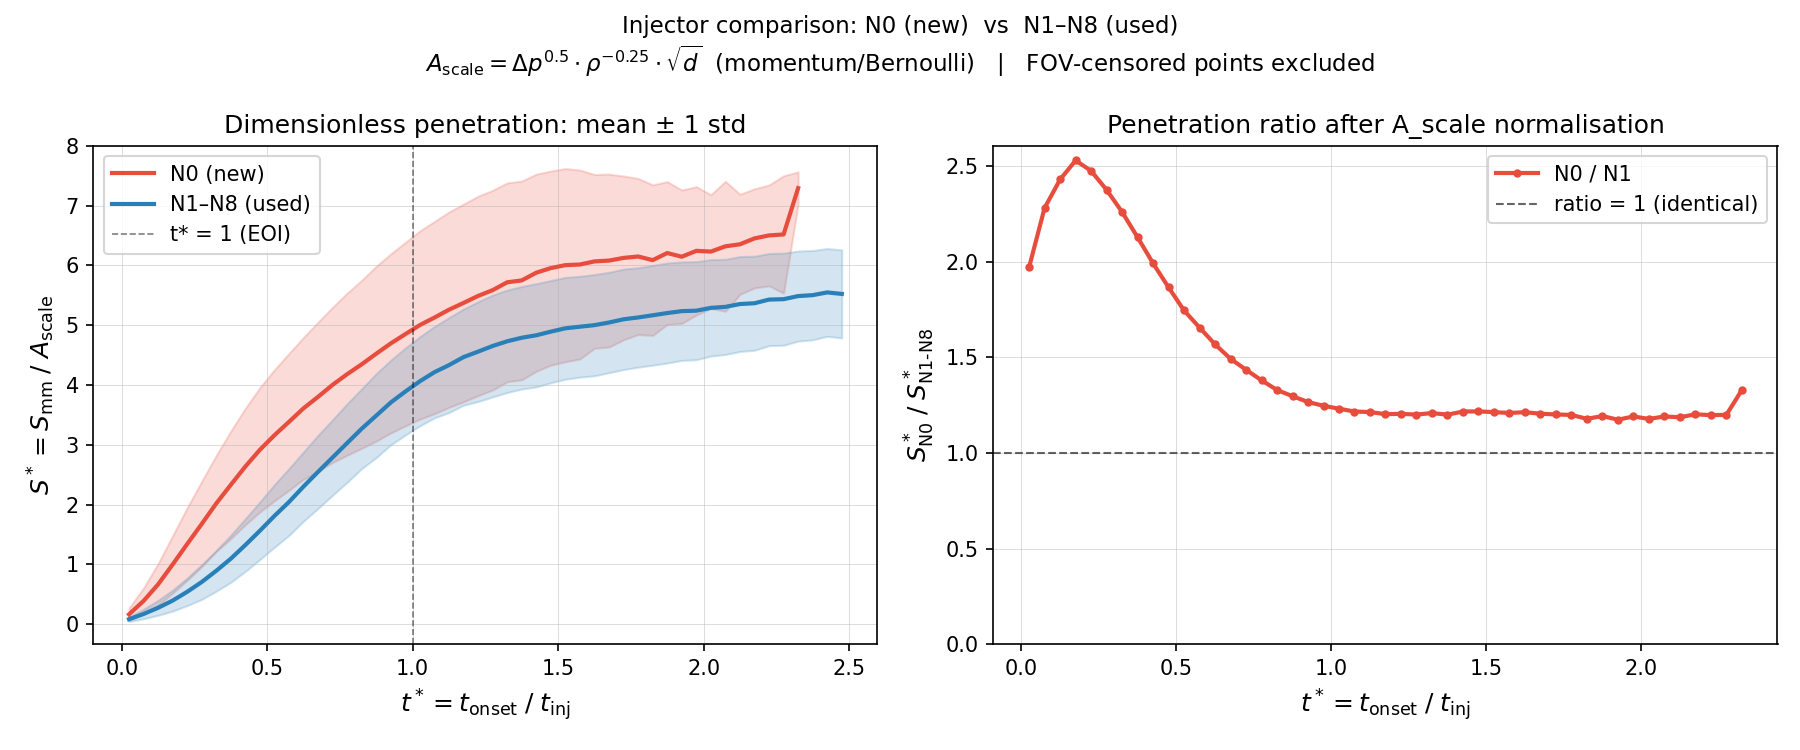
\includegraphics[height=0.58\textheight,keepaspectratio]{figs/injector_comparison_dp050.png}
\end{center}
\vspace{-0.15em}
\scriptsize
\begin{itemize}\setlength\itemsep{1pt}
  \item Even after momentum/Bernoulli-style normalisation, N0 remains distinct:
        early-time response reaches \warn{$\sim$2.5$\times$} N1--N8 and stays above 1.
  \item N0 is a \textbf{cross-injector-distribution} problem, not merely a missing
        per-family output head.
\end{itemize}
\end{frame}

% ------------------------------------------------------------------
\begin{frame}{Evidence: the full scatter separates N0's early branch}
\small
\begin{center}

\includegraphics[height=0.66\textheight,keepaspectratio]{figs/injector_scatter_all_nozzles.png}
\end{center}
\vspace{-0.15em}
\scriptsize
\centering
Nozzle0 occupies a higher early-time envelope before and around \(t^\ast=1\), while
the used injectors mostly overlap. The residual head can remove a family offset, but
it cannot create a trunk representation for a branch the frozen backbone never saw.
\end{frame}

% ------------------------------------------------------------------
\begin{frame}{N6 and N0: two faces of out-of-design-family}
\small
The residual head's structural fallback works \emph{when the new family is in design
family}. Two cases mark the boundary:

\vspace{0.3em}
\begin{columns}[T]
\column{0.5\textwidth}
\begin{block}{Nozzle6 (LONO stress fold)}
Data-sparsest fold (20k points). All MLP arms collapse to 12--14 mm; the residual
arms are \warn{2.3 mm worse} than the family head and under-predict (bias $-10.5$).
Specialisation \emph{over-commits} on a family the trunk barely supports.
\end{block}

\column{0.5\textwidth}
\begin{block}{Nozzle0 (the genuine new injector)}
The only first-generation (BC2022) injector --- same orifice geometry, empirically
distinct signature. Zero-shot (trunk never saw N0): \warn{33.16 mm}. The deployment
question: how many N0 conditions does the per-family delta head need to recover?
\end{block}
\end{columns}

\vspace{0.4em}
\footnotesize
Both echo the thesis' Nozzle0 cross-design-family failure: a per-family \emph{output}
correction cannot synthesise a representation the frozen trunk never learned.
\end{frame}

% ------------------------------------------------------------------
\begin{frame}{N0 few-shot adaptation: the limit, quantified}
\small
\begin{columns}[T]
\column{0.54\textwidth}
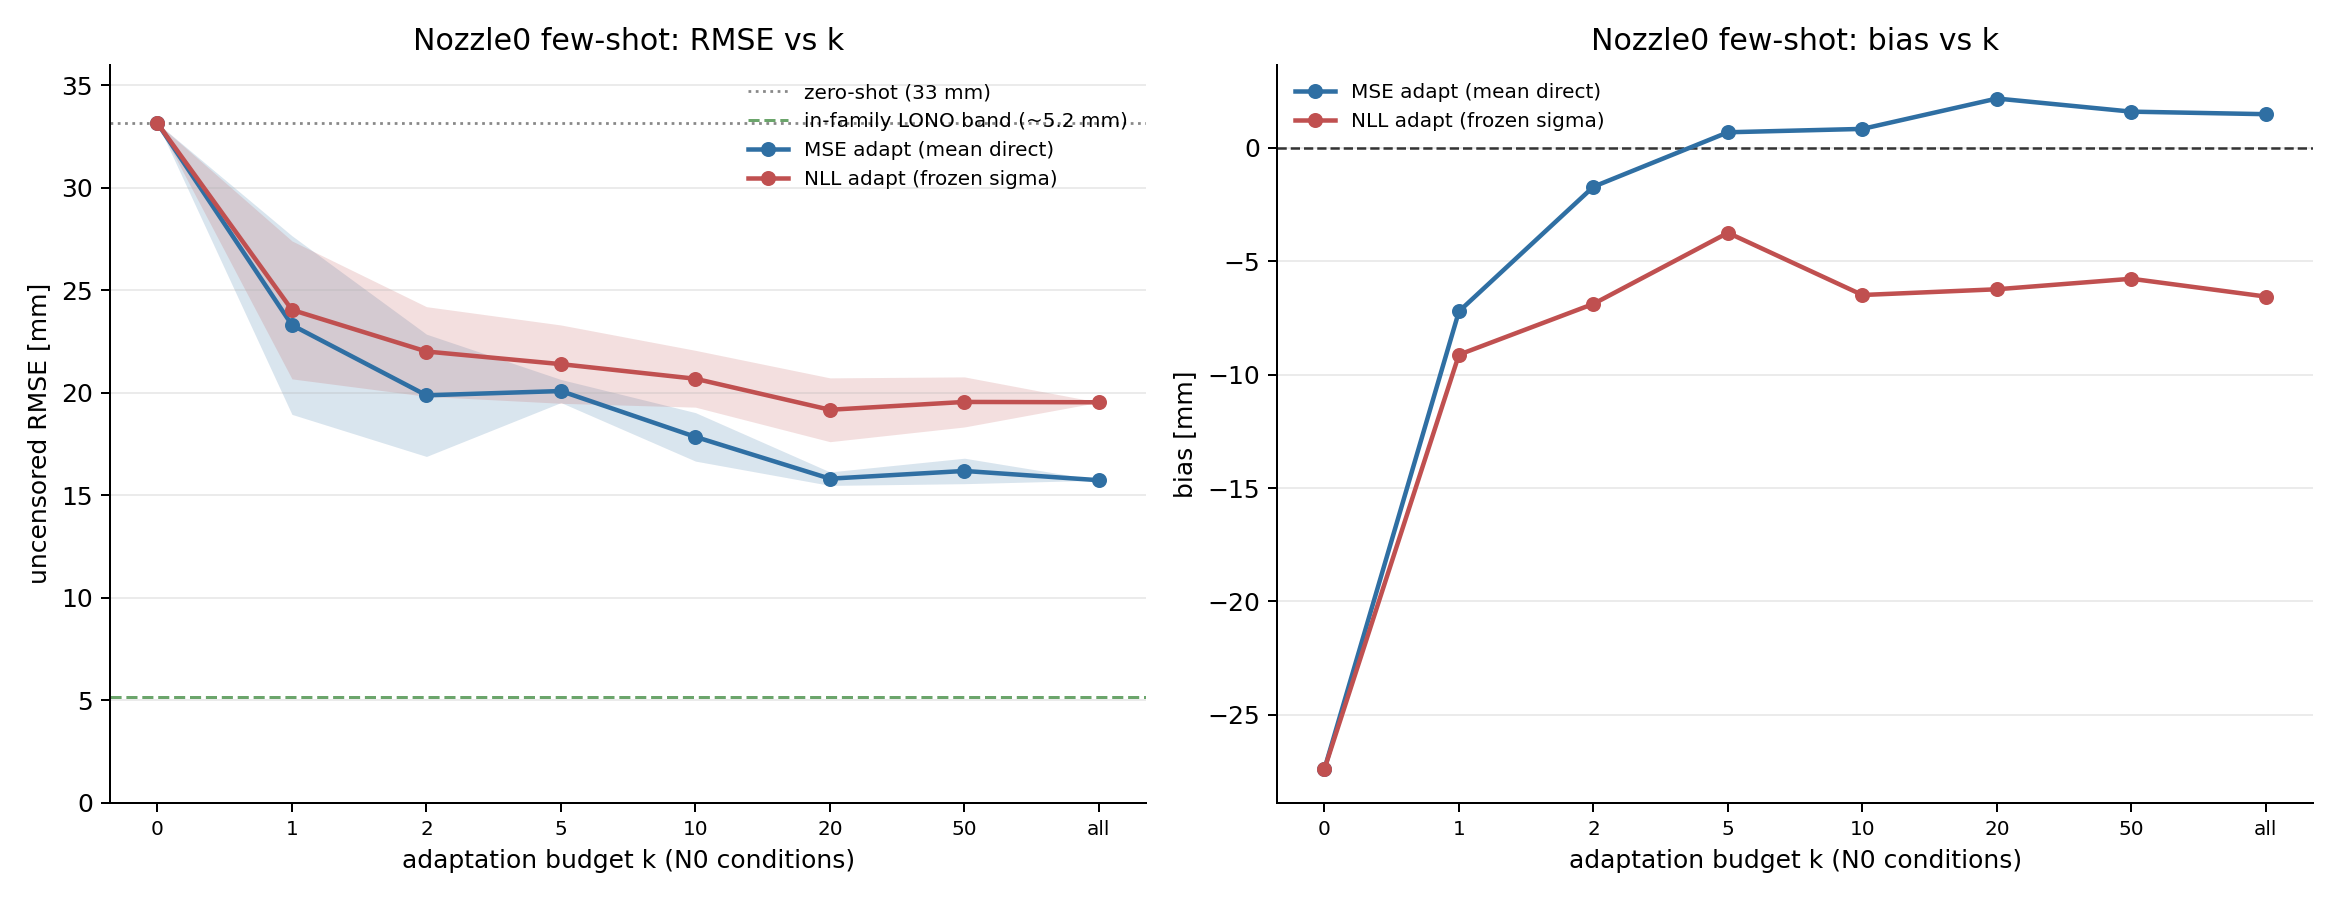
\includegraphics[width=\linewidth]{figs/n0_fewshot_adaptation_curve.png}
\column{0.46\textwidth}
\scriptsize
Freeze everything except \texttt{delta\_heads[0]}; fine-tune on $k$ N0 conditions;
evaluate uncensored RMSE (in-family LONO band $\approx$5 mm).
\vspace{0.3em}
\begin{tabular}{@{}rrr@{}}
\toprule
$k$ & NLL & MSE \\
\midrule
0 (zero-shot) & 33.16 & 33.16 \\
2  & 22.01 & 19.88 \\
10 & 20.68 & 17.85 \\
20 & 19.17 & 15.81 \\
all (203) & 19.54 & \textbf{15.73} \\
\bottomrule
\end{tabular}
\column{0.0\textwidth}
\end{columns}

\vspace{0.4em}
\begin{enumerate}\setlength\itemsep{2pt}
  \item \textbf{The frozen variance head throttles NLL adaptation.} On OOD N0 the
        frozen log-var emits a huge $\sigma$ (mean std $\sim$1443 mm at $k{=}0$),
        down-weighting the mean gradient. Fitting the mean directly (MSE) drops the
        floor by \good{$\sim$4 mm} and removes the bias by $k{=}2$.
  \item \textbf{Even unthrottled, delta-only adaptation plateaus at $\sim$15.7 mm}
        --- far above the $\sim$5 mm in-family band. A per-family offset removes the
        global bias but \warn{cannot close the residual spread}: N0 needs trunk-level
        capacity (unfreeze / FiLM-all-blocks / retrain), not a new output head.
\end{enumerate}
\end{frame}

% ==================================================================
\section{Significance and synthesis}

% ------------------------------------------------------------------
\begin{frame}{What this adds to the thesis}
\small
\begin{enumerate}\setlength\itemsep{5pt}
  \item \textbf{A new best on the primary table.} The residual multi-task SVGP reaches
        \good{3.987 mm} CDF and \good{2.077 mm} P50 on the same uncensored table ---
        beating the thesis' strongest model (SVGP 4.193 / P50 2.649) by $\sim$5\% on
        CDF RMSE and \good{0.57 mm} on P50. QC-gated retraining still improves when
        re-scored on lv2 (\good{3.922 / 1.912}) and reaches \good{3.848 / 1.829} on
        lv3; the latter is sensitivity evidence, not the sole final proof.
  \item \textbf{The deployment gap is closed structurally --- within design family.}
        A new injector family is a zero-initialised residual that \emph{automatically}
        falls back to the shared model --- no hard-coded fallback identity, no retrain,
        $\sim$50k trainable params on a frozen backbone. The fallback is mechanically
        clean for \emph{any} family but predictively safe only in-design-family
        (the N0/N6 boundary).
  \item \textbf{The MLP branch's LONO weakness is partly repaired.} The residual
        conversion turns the family head's $+5$ mm over-prediction into $+0.78$ mm and
        cuts in-family LONO RMSE by 31\% --- directly strengthening Chapter 5's
        transfer story for the MLP stack.
  \item \textbf{The boundary is drawn honestly.} N6/N0 show the cheap adapter recovers
        in-design-family injectors but not out-of-design-family ones --- a constructive,
        quantified refinement of the thesis' Nozzle0 failure rather than a hidden caveat.
\end{enumerate}
\end{frame}

% ------------------------------------------------------------------
\begin{frame}{Verdict and next steps}
\small
\begin{block}{Verdict}
The single principle --- \emph{additive residual on a hot-started, frozen backbone} ---
upgrades the deployed surrogate along both axes the thesis left open: it makes the
model cleanly extensible to new families \emph{and}, on the SVGP backbone, sets a new
accuracy/calibration best on the primary uncensored CDF table, all while preserving
the auditable deployment path.
\end{block}

\vspace{0.3em}
\begin{itemize}\setlength\itemsep{2pt}
  \item Package the residual SVGP as the candidate deployed model, with the QC-gated
        checkpoint as the current strongest sensitivity row; keep residual-FiLM as the
        best MLP-only option and residual FH as the simplest
        fallback. \emph{Caveat:} LONO transfer is validated for the MLP arms only;
        the residual SVGP's LONO behaviour is unmeasured here, though the thesis SVGP
        already out-transfers the MLP (5.95 vs 7.00 mm excl.\ N0) --- confirm with a
        residual-SVGP LONO fold.
  \item For genuinely new injectors: adapt the log-var head alongside the delta, and
        test trunk-level capacity (FiLM-all-blocks / last-block unfreeze) to close the
        N0/N6 residual spread.
\end{itemize}

\vspace{0.3em}
\scriptsize
\textbf{Artifacts:}
\texttt{residual\_from\_prod\_eval\_summary.csv};
\texttt{residual\_svgp\_vs\_latest\_mlp.csv};
\texttt{lono\_modified\_only/};
\texttt{dataset\_ablation\_qc\_gated/};
\texttt{cross\_dataset\_lv2\_lv3/};
\texttt{n0\_fewshot\_adaptation/}; figures under \texttt{figs/}.
\end{frame}


% ==================================================================
\appendix
\section{Backup: in-distribution training detail}


% ------------------------------------------------------------------
\begin{frame}{Training log read}
\small
\begin{center}
\renewcommand{\arraystretch}{1.15}
\setlength{\tabcolsep}{5pt}
\begin{tabular}{@{}lrrrr@{}}
\toprule
\textbf{delta L2} & \textbf{mimic epochs} & \textbf{stop epoch} & \textbf{test loss} & \textbf{test delta RMS} \\
\midrule
0      & 10 & 104 & 2.074 & 0.816 \\
1e-4   & 10 & 44  & 2.085 & 0.818 \\
1e-3   & 10 & 110 & 2.070 & 0.813 \\
1e-2   & 10 & 84  & 2.083 & 0.810 \\
\bottomrule
\end{tabular}
\end{center}

\vspace{0.6em}
\begin{itemize}\setlength\itemsep{2pt}
  \item All four runs completed and early-stopped cleanly.
  \item The mimic stage reduced the initial production-head mismatch before raw refinement.
  \item Delta magnitudes stayed tightly clustered (\(\mathrm{RMS}\approx0.81\) in
        A-scaled space), so the shrinkage sweep mainly changes calibration and tail
        behaviour, not gross residual size.
\end{itemize}
\end{frame}

% ------------------------------------------------------------------
\begin{frame}{Step 1 --- Residual head beats the deployed family head}
\small
\begin{center}
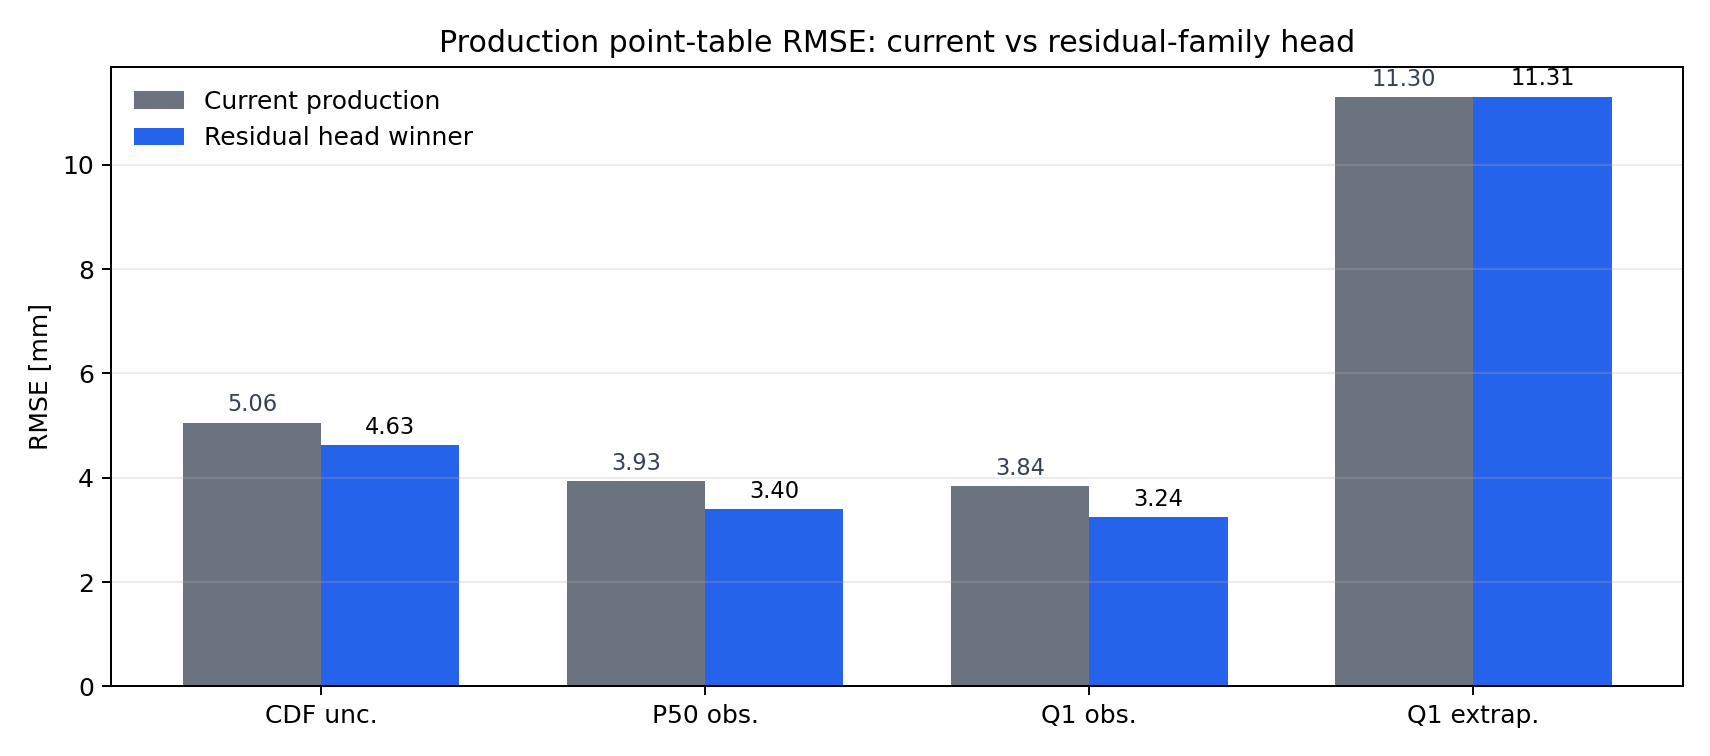
\includegraphics[width=0.56\textwidth]{figs/production_rmse_comparison.png}
\end{center}
\vspace{-0.4em}
\begin{center}
\scriptsize
\renewcommand{\arraystretch}{1.08}
\setlength{\tabcolsep}{5pt}
\begin{tabular}{@{}lrrrrr@{}}
\toprule
\textbf{Model} & \textbf{CDF RMSE} & \textbf{CDF ECE} & \textbf{CDF CRPS} & \textbf{P50 RMSE} & \textbf{Q1 obs RMSE} \\
\midrule
Deployed family head & 5.056 & 0.0708 & 2.801 & 3.931 & 3.839 \\
\rowcolor{winrow}
Residual winner (1e-4) & \textbf{4.631} & \textbf{0.0604} & \textbf{2.382} & \textbf{3.395} & \textbf{3.242} \\
\bottomrule
\end{tabular}
\end{center}
\vspace{0.2em}
\footnotesize
\centering
CDF RMSE \good{$-0.425$ mm}, bias toward zero \good{($+0.343\to+0.180$)},
calibration \good{(ECE $0.0708\to0.0604$, CRPS $2.801\to2.382$)}.
\end{frame}

% ------------------------------------------------------------------
\begin{frame}{Step 1 --- shrinkage sweep and per-point deltas}
\small
\begin{columns}[T]
\column{0.52\textwidth}
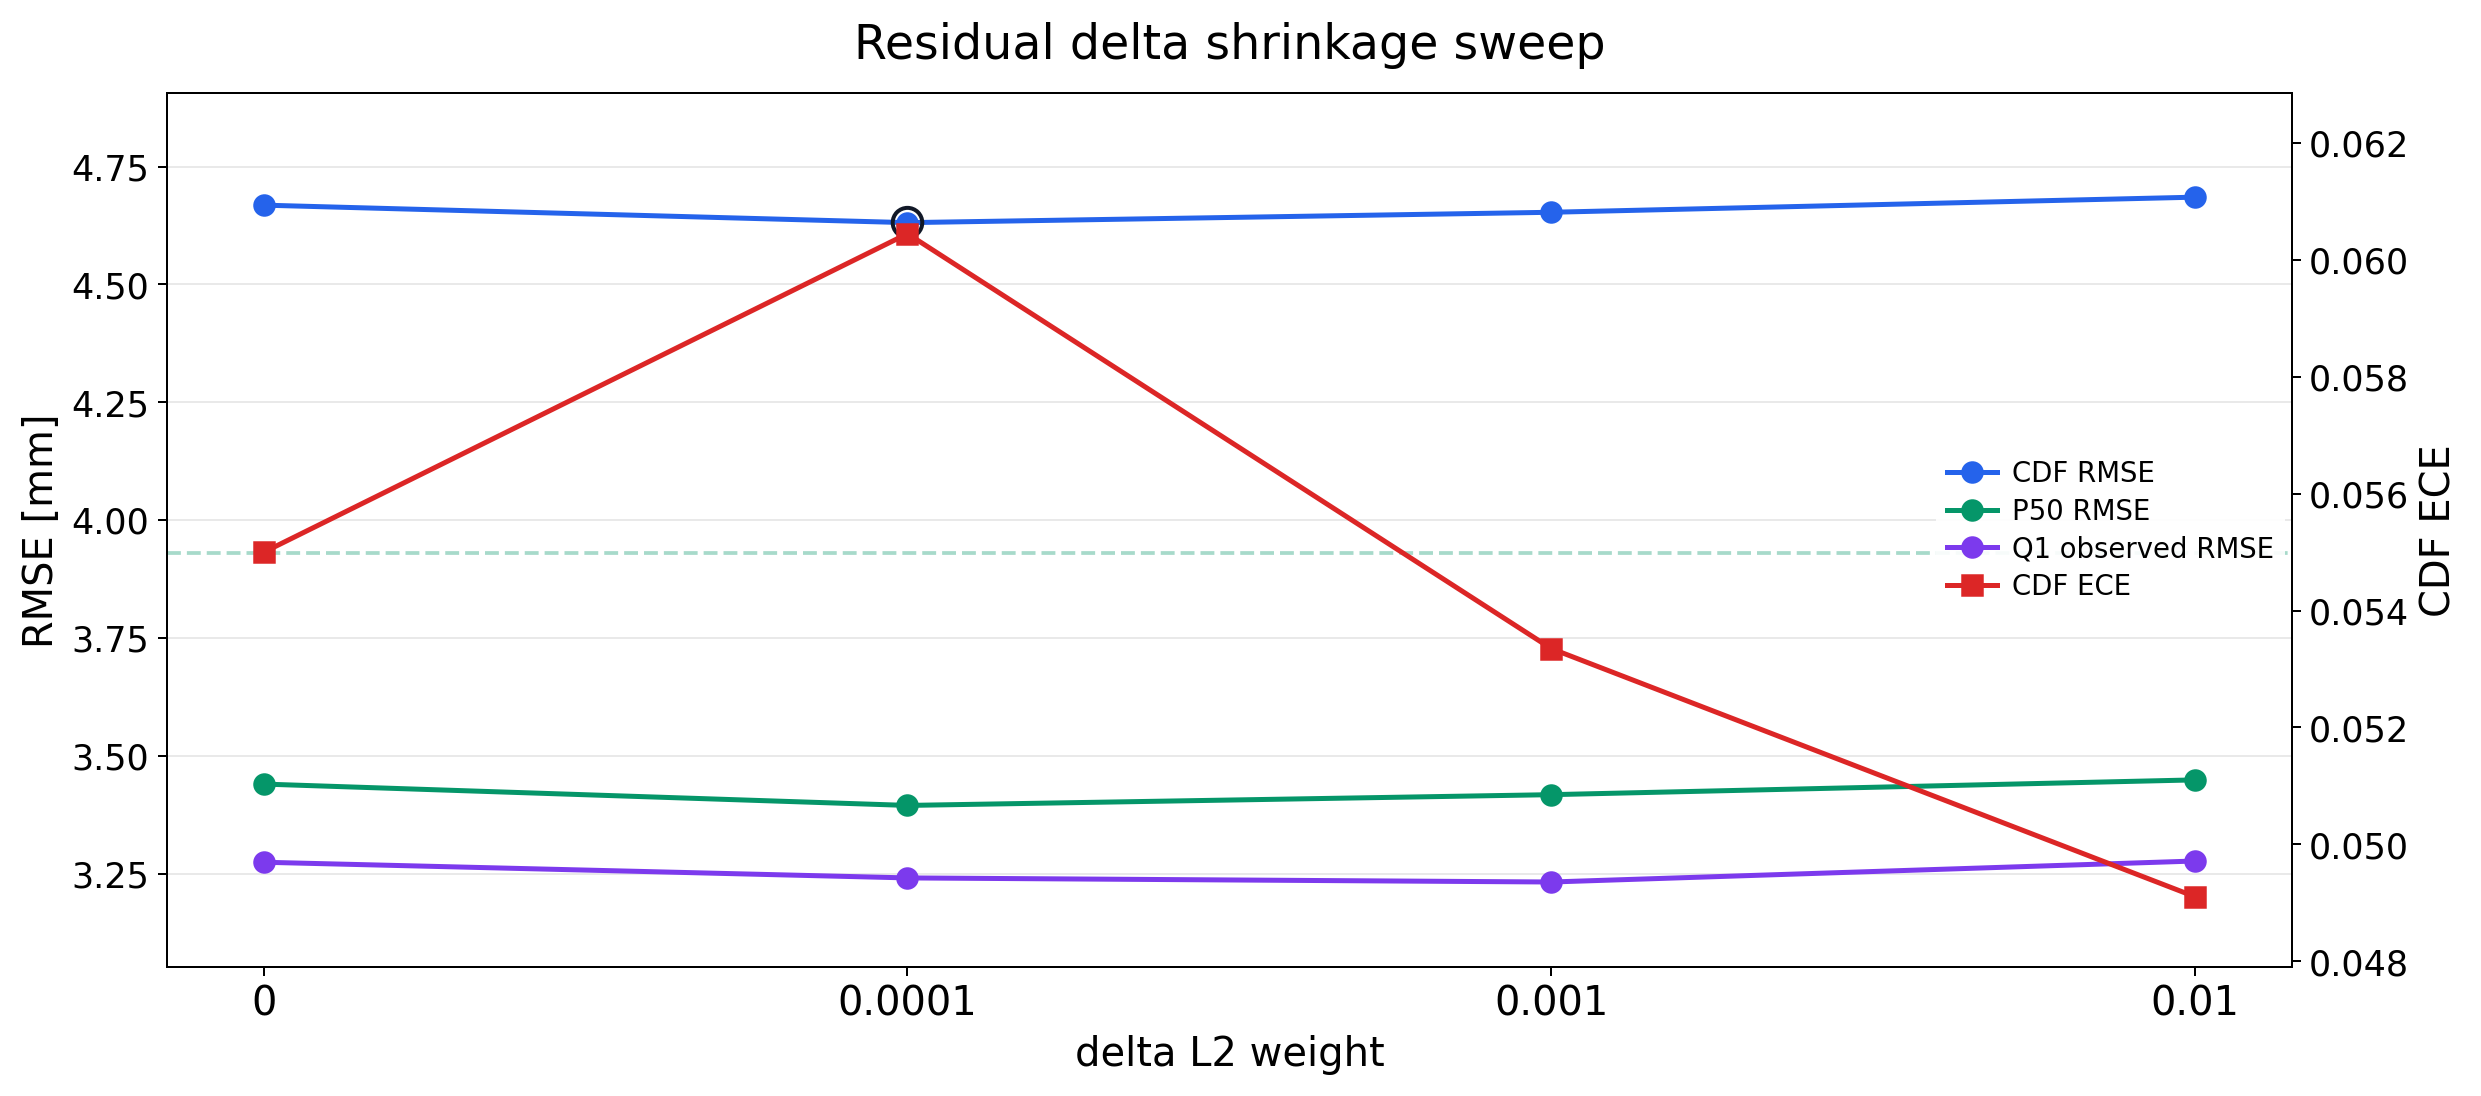
\includegraphics[width=\linewidth]{figs/delta_l2_sweep.png}
\column{0.48\textwidth}
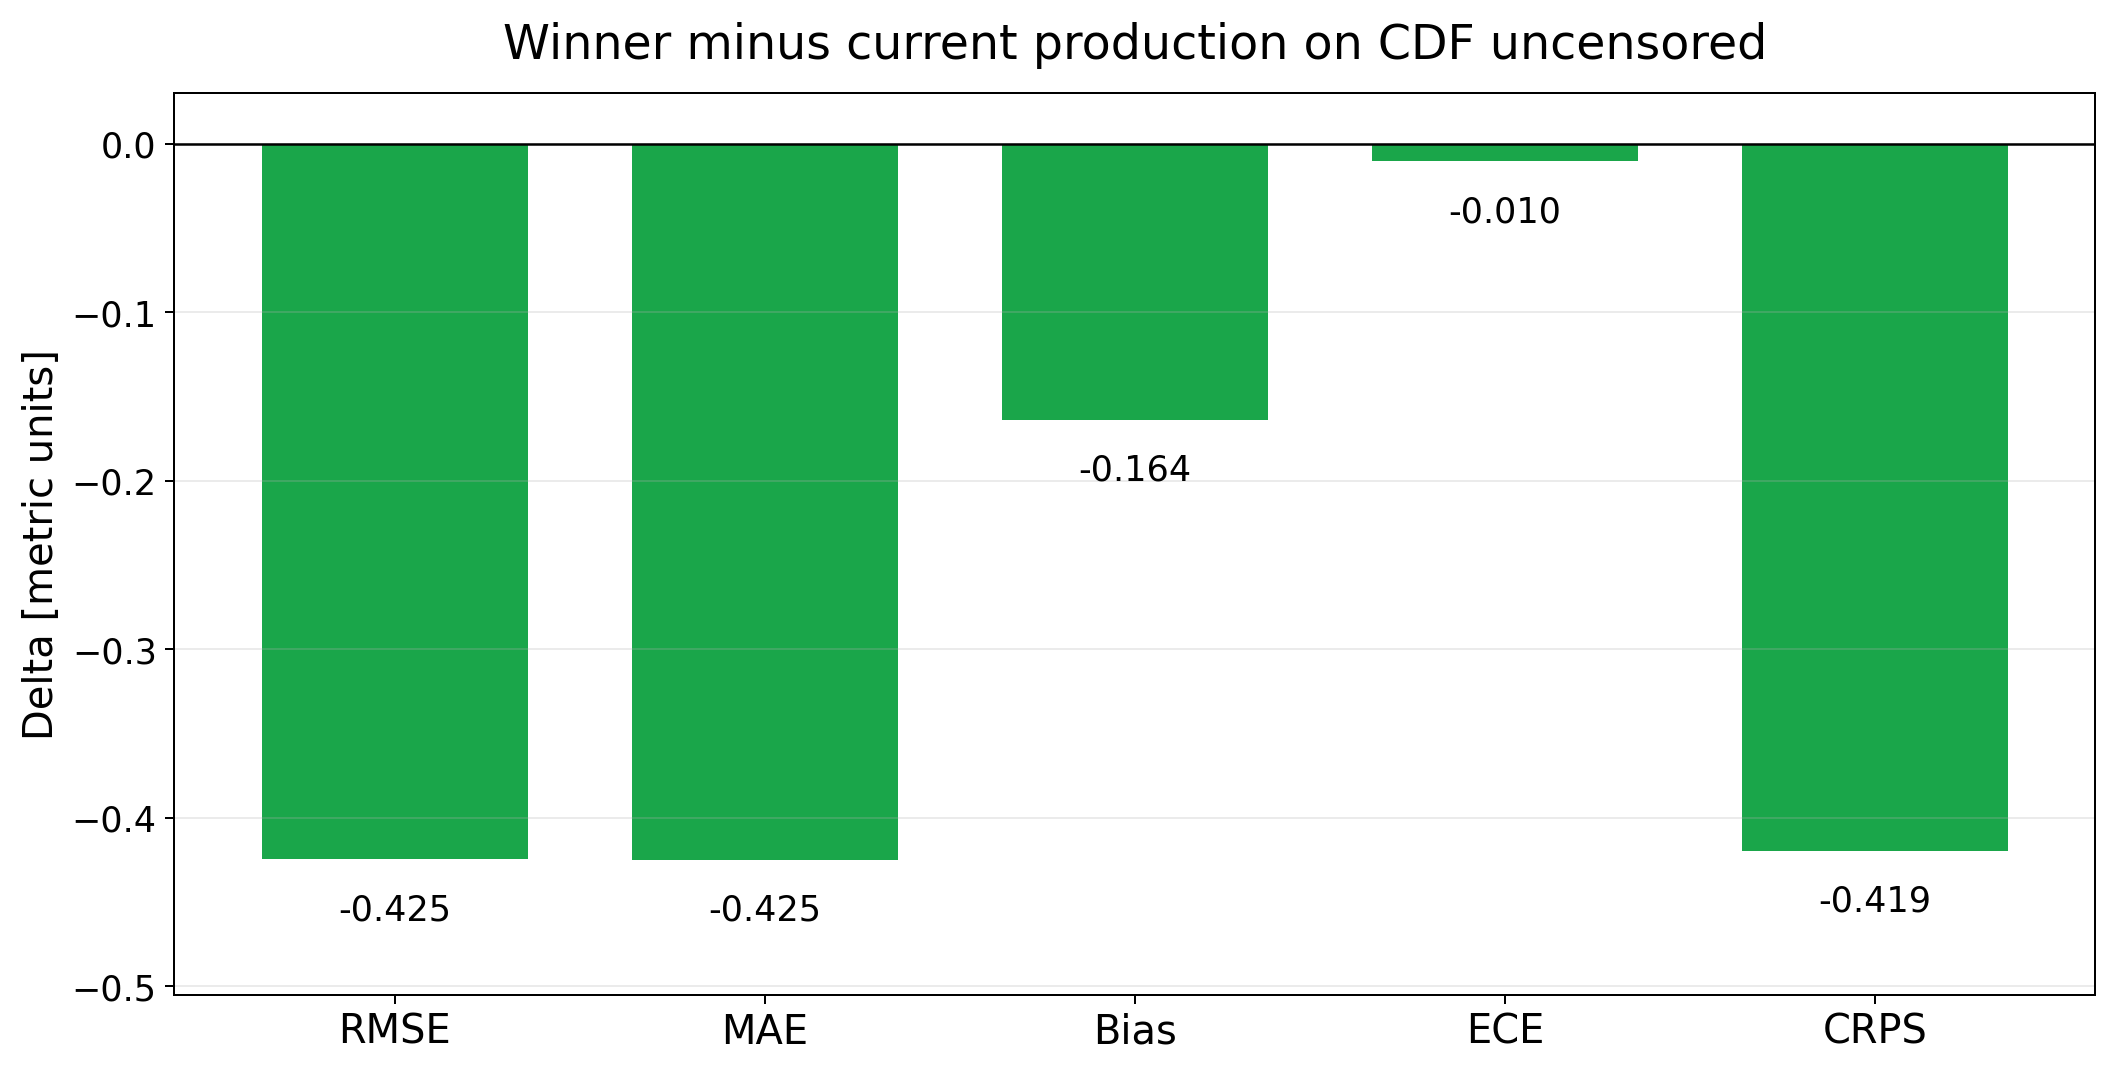
\includegraphics[width=\linewidth]{figs/winner_cdf_deltas.png}
\end{columns}
\vspace{0.3em}
\begin{itemize}\setlength\itemsep{2pt}
  \item \emph{All} residual settings beat the deployed family head on CDF RMSE;
        \texttt{1e-4} gives the best primary RMSE \good{(4.631 mm)}.
  \item Stronger shrinkage improves ECE and extrapolated Q1 but gives back a little
        primary RMSE --- the sweep is a calibration/tail knob.
\end{itemize}
\end{frame}

% ------------------------------------------------------------------
\begin{frame}{Step 2 --- FiLM: the family signal is partly representational}
\small
The recommended MLP-only ablation, run on production (no LONO): an identity FiLM
adapter after the final trunk block, hot-started from the residual family head, trunk
and shared mean frozen.

\vspace{0.2em}
\begin{center}
\scriptsize
\renewcommand{\arraystretch}{1.14}
\setlength{\tabcolsep}{3.4pt}
\begin{tabular}{@{}lrrrrrrr@{}}
\toprule
\textbf{Model} & \textbf{film L2} & \textbf{delta L2} & \textbf{CDF RMSE} & \textbf{CDF ECE} & \textbf{CDF CRPS} & \textbf{P50 RMSE} & \textbf{Q1 obs RMSE} \\
\midrule
Source residual FH & -- & \texttt{1e-2} & 4.685 & 0.0491 & 2.368 & 3.449 & 3.277 \\
\rowcolor{winrow}
Residual-FiLM & \texttt{1e-4} & \texttt{1e-3} & \textbf{4.510} & \textbf{0.0404} & \textbf{2.242} & \textbf{3.166} & \textbf{3.110} \\
\bottomrule
\end{tabular}
\end{center}

\vspace{0.35em}
\begin{itemize}\setlength\itemsep{2pt}
  \item CDF RMSE \good{$-0.176$ mm}; P50 \good{$-0.283$ mm}; ECE $0.0491\to0.0404$,
        CRPS $2.368\to2.242$; Q1 extrapolated effectively flat ($11.248\to11.265$).
  \item All nine \texttt{(film,delta)} settings beat the source residual head:
        family difference is useful as a hidden-representation modulation, not only
        as an output offset.
\end{itemize}
\end{frame}

% ------------------------------------------------------------------
\begin{frame}{Step 3 --- Additive-residual multi-task SVGP: new best}
\small
The same additive-residual idea on the probabilistic backbone: a shared SVGP
hot-started from the deployed Stage-3 checkpoint $+$ per-family residual GPs, family
id outside the kernel, zero-residual fallback for unseen families.

\vspace{0.2em}
\begin{center}
\scriptsize
\renewcommand{\arraystretch}{1.14}
\setlength{\tabcolsep}{3.4pt}
\begin{tabular}{@{}lrrrrrr@{}}
\toprule
\textbf{Model} & \textbf{delta L2} & \textbf{CDF RMSE} & \textbf{CDF ECE} & \textbf{CDF CRPS} & \textbf{P50 RMSE} & \textbf{Q1 extrap RMSE} \\
\midrule
MLP residual FH & \texttt{1e-2} & 4.685 & 0.0491 & 2.368 & 3.449 & 11.248 \\
\rowcolor{winrow}
Residual SVGP & \texttt{1e-4} & \textbf{3.987} & \textbf{0.0262} & \textbf{2.040} & \textbf{2.077} & \textbf{10.429} \\
\bottomrule
\end{tabular}
\end{center}

\vspace{0.35em}
\begin{itemize}\setlength\itemsep{2pt}
  \item Beats the single-output SVGP baseline (CDF $4.193\to3.987$) --- and the
        probabilistic backbone halves ECE vs the residual MLP (\good{0.026} vs 0.060).
  \item A narrow, stable shrinkage sweep: \texttt{1e-4} is the sweet spot for primary
        RMSE \emph{and} calibration on the evaluated tables.
\end{itemize}
\end{frame}

% ------------------------------------------------------------------
\begin{frame}{Step 3 --- Residual SVGP vs current best}
\small
\begin{center}
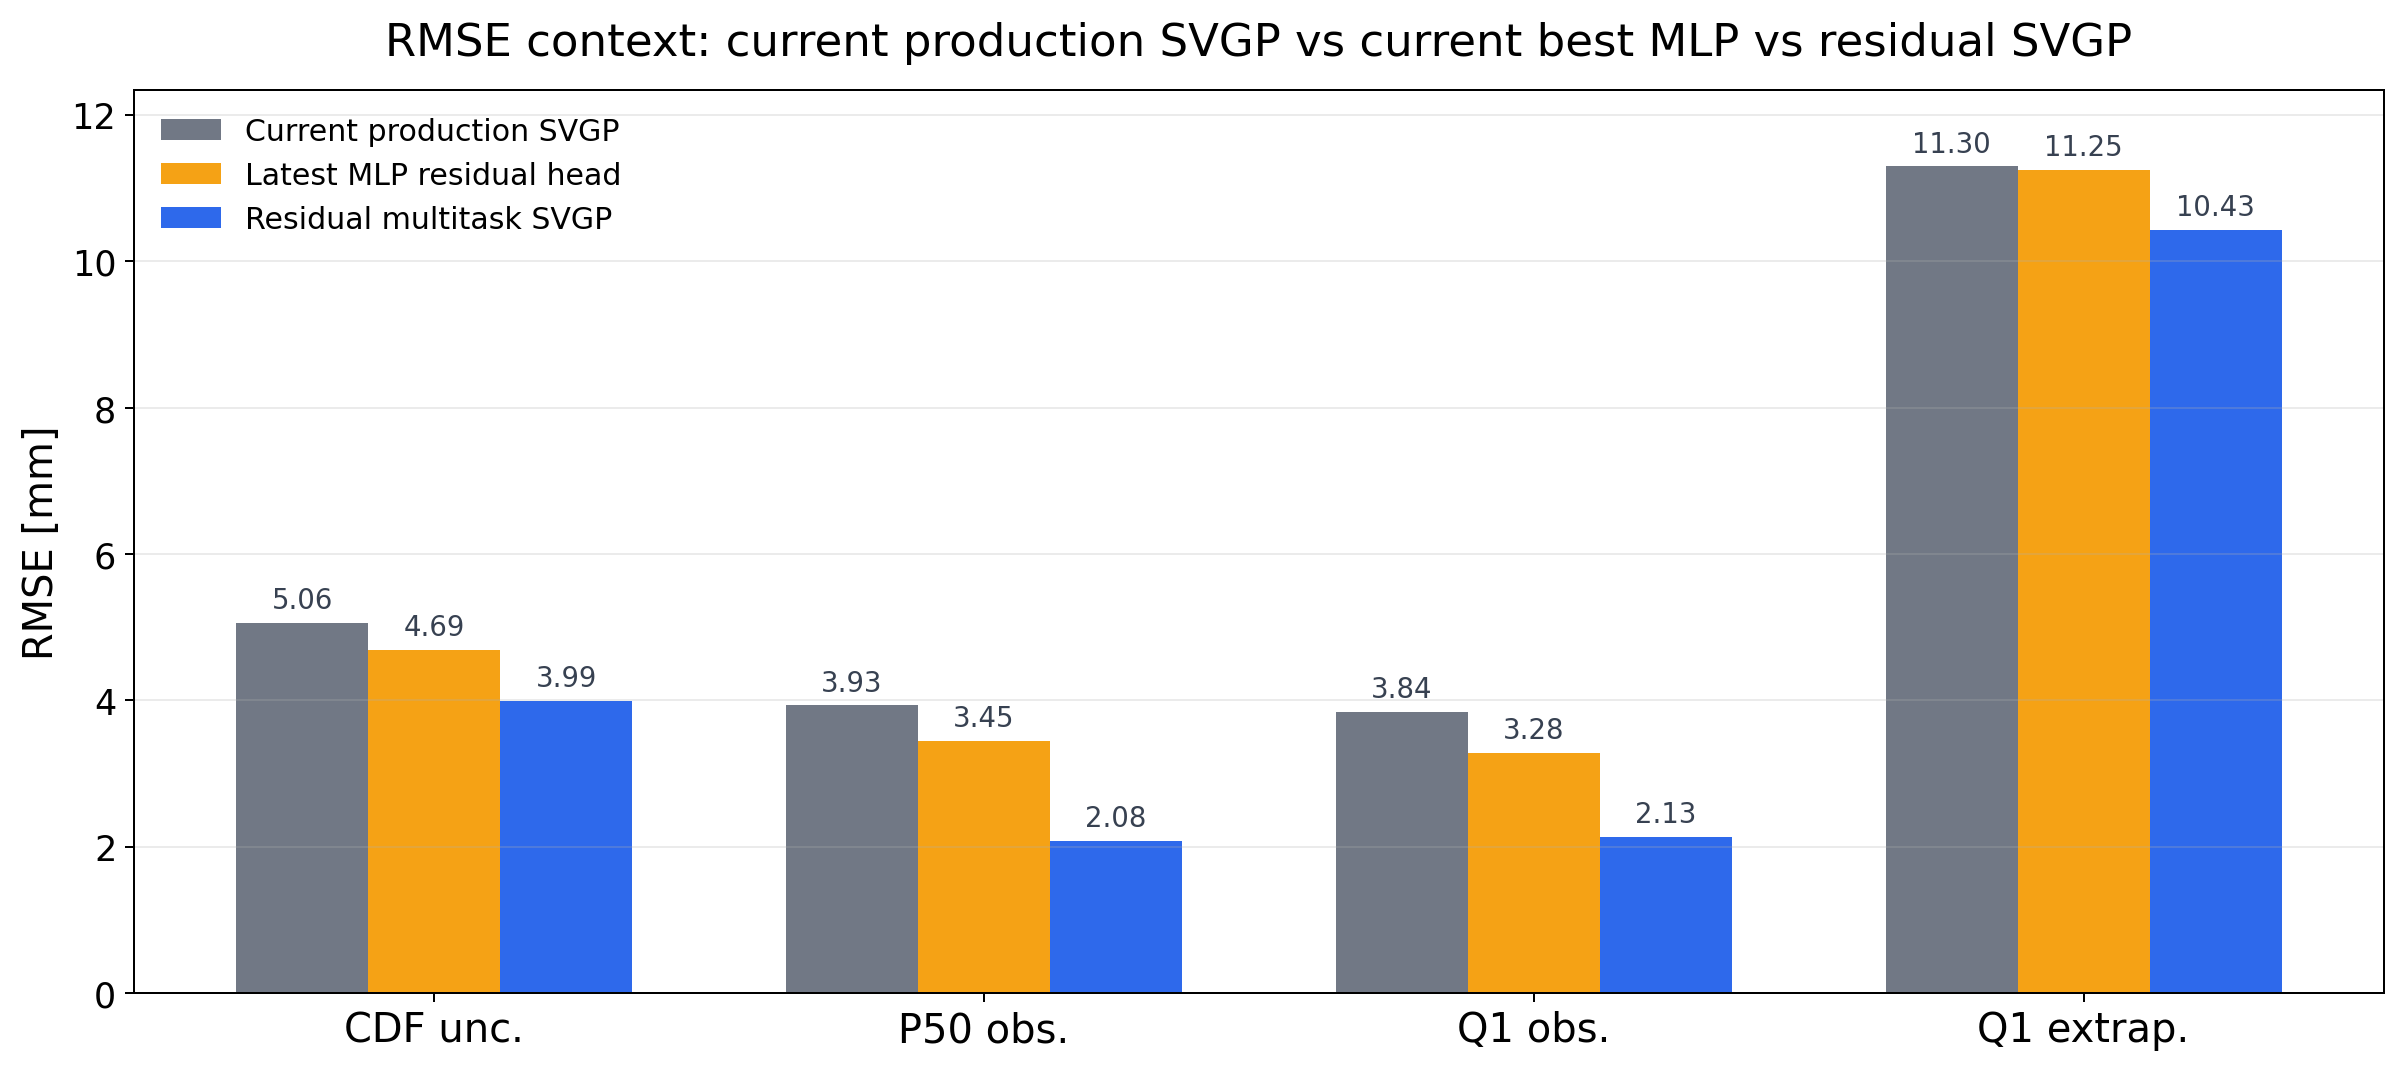
\includegraphics[width=0.90\textwidth]{figs/residual_svgp_context_rmse_comparison.png}
\end{center}
\end{frame}

% ------------------------------------------------------------------
\begin{frame}{The climb on one table (uncensored CDF, lv2 542k points)}
\small
\begin{center}
\renewcommand{\arraystretch}{1.18}
\setlength{\tabcolsep}{6pt}
\begin{tabular}{@{}lrrl@{}}
\toprule
\textbf{Model} & \textbf{CDF RMSE} & \textbf{P50 RMSE} & \textbf{Origin} \\
\midrule
Naber--Siebers (physics)            & 9.286 & -- & thesis \\
Three-stage MLP, selected surrogate & 4.265 & 2.848 & thesis \\
Stage-3 SVGP                        & 4.193 & 2.649 & thesis (prev.\ best) \\
\midrule
Deployed family head                & 5.010 & 3.907 & deployment variant \\
Residual FH (1e-4)                  & 4.631 & 3.395 & \textbf{this work} \\
Residual-FiLM                       & 4.510 & 3.166 & \textbf{this work} \\
\rowcolor{winrow}
Residual SVGP (1e-4)                & \textbf{3.987} & \textbf{2.077} & \textbf{this work (new best)} \\
Residual SVGP, QC-gated retrain     & 3.922 & 1.912 & sensitivity re-score \\
\bottomrule
\end{tabular}
\end{center}
\vspace{0.3em}
\footnotesize
\textbf{Read honestly:} the residual \emph{MLP} (4.631) recovers most of the accuracy
the per-family head gave up (5.010) but does \emph{not} beat the simpler single-head
surrogate (4.265). The structural accuracy frontier is advanced by the residual
\emph{SVGP} (\good{3.987}), which beats the thesis' strongest model (4.193). The
QC-gated retrain improves the residual SVGP again on the same lv2 root
(\good{3.987$\to$3.922}) but is treated as a sensitivity result, not the sole proof.
\end{frame}

\end{document}
